\documentclass[11,]{article}
\usepackage{lmodern}
\usepackage{amssymb,amsmath}
\usepackage{ifxetex,ifluatex}
\usepackage{fixltx2e} % provides \textsubscript
\ifnum 0\ifxetex 1\fi\ifluatex 1\fi=0 % if pdftex
  \usepackage[T1]{fontenc}
  \usepackage[utf8]{inputenc}
\else % if luatex or xelatex
  \ifxetex
    \usepackage{mathspec}
  \else
    \usepackage{fontspec}
  \fi
  \defaultfontfeatures{Ligatures=TeX,Scale=MatchLowercase}
\fi
% use upquote if available, for straight quotes in verbatim environments
\IfFileExists{upquote.sty}{\usepackage{upquote}}{}
% use microtype if available
\IfFileExists{microtype.sty}{%
\usepackage{microtype}
\UseMicrotypeSet[protrusion]{basicmath} % disable protrusion for tt fonts
}{}
\usepackage[margin=1in]{geometry}
\usepackage{hyperref}
\PassOptionsToPackage{usenames,dvipsnames}{color} % color is loaded by hyperref
\hypersetup{unicode=true,
            colorlinks=true,
            linkcolor=Maroon,
            citecolor=Blue,
            urlcolor=blue,
            breaklinks=true}
\urlstyle{same}  % don't use monospace font for urls
\usepackage{longtable,booktabs}
\usepackage{graphicx,grffile}
\makeatletter
\def\maxwidth{\ifdim\Gin@nat@width>\linewidth\linewidth\else\Gin@nat@width\fi}
\def\maxheight{\ifdim\Gin@nat@height>\textheight\textheight\else\Gin@nat@height\fi}
\makeatother
% Scale images if necessary, so that they will not overflow the page
% margins by default, and it is still possible to overwrite the defaults
% using explicit options in \includegraphics[width, height, ...]{}
\setkeys{Gin}{width=\maxwidth,height=\maxheight,keepaspectratio}
\IfFileExists{parskip.sty}{%
\usepackage{parskip}
}{% else
\setlength{\parindent}{0pt}
\setlength{\parskip}{6pt plus 2pt minus 1pt}
}
\setlength{\emergencystretch}{3em}  % prevent overfull lines
\providecommand{\tightlist}{%
  \setlength{\itemsep}{0pt}\setlength{\parskip}{0pt}}
\setcounter{secnumdepth}{5}
% Redefines (sub)paragraphs to behave more like sections
\ifx\paragraph\undefined\else
\let\oldparagraph\paragraph
\renewcommand{\paragraph}[1]{\oldparagraph{#1}\mbox{}}
\fi
\ifx\subparagraph\undefined\else
\let\oldsubparagraph\subparagraph
\renewcommand{\subparagraph}[1]{\oldsubparagraph{#1}\mbox{}}
\fi

%%% Use protect on footnotes to avoid problems with footnotes in titles
\let\rmarkdownfootnote\footnote%
\def\footnote{\protect\rmarkdownfootnote}

%%% Change title format to be more compact
\usepackage{titling}

% Create subtitle command for use in maketitle
\providecommand{\subtitle}[1]{
  \posttitle{
    \begin{center}\large#1\end{center}
    }
}

\setlength{\droptitle}{-2em}

  \title{}
    \pretitle{\vspace{\droptitle}}
  \posttitle{}
    \author{}
    \preauthor{}\postauthor{}
    \date{}
    \predate{}\postdate{}
  
%%% .rmd + .sty setup borrowed from: https://github.com/oganm/ThesisProposal

% Must load tex packages here (import.sty run in preamble, title.sty run after)
\usepackage{setspace} % for title page spacing
\usepackage{hyperref} % for all sorts of linking

\begin{document}

%%% .rmd + .sty setup borrowed from: https://github.com/oganm/ThesisProposal

\onehalfspacing
\pagenumbering{gobble}

%\begin{titlepage}
\begin{center}
\LARGE{\textbf{Dynamic visualization of high-dimensional data via
low-dimension projections and sectioning across 2D and 3D display devices}}\\
\vspace*{2\baselineskip}
\Large{\textbf{Mid canidature review}}\\
\normalsize{Monash University, Faculty of Information Technology}\\
\vspace*{2\baselineskip}
\Large{Nicholas Spyrison}\\ %, B.Sc
\vspace*{3\baselineskip}
\Large{\textbf{Thesis Supervisors}}\\
Prof. Kimbal Marriott\\
Prof. Dianne Cook\\
\vspace*{2\baselineskip}
\Large{\textbf{Committee Members}}\\
Dr. Maxime Cordiel\\
Dr. Shirui Pan\\
\vspace*{1\baselineskip}
\Large{\textbf{Chair}}\\
Assoc. Prof. Bernhard Jenny\\
\vspace*{1\baselineskip}
\Large{\textbf{Presention Date}}\\
DD Feburuary, 2020
\end{center}
% \end{titlepage}

\doublespacing

\hypersetup{linkcolor = blue}
\newpage
\pagenumbering{roman}
\tableofcontents
\addcontentsline{toc}{section}{\contentsname}

\newpage

%% list of figures have to be added manually to table of contents
% \listoffigures 
% 
% \newpage
% \listoftables

\doublespacing

\newpage
\pagenumbering{arabic}
\hypersetup{linkcolor = blue}

{
\hypersetup{linkcolor=black}
\setcounter{tocdepth}{2}
\tableofcontents
}
\hypertarget{sec:intro}{%
\section{Introduction}\label{sec:intro}}

\hypertarget{exploratory-data-analysis}{%
\subsection{Exploratory data analysis}\label{exploratory-data-analysis}}

The term exploratory data analysis was coined by Tukey (1977), who leaves it as an intentionally broad term which encompasses the initial summarization and visualization of a data set. This is a critical first step of checking for realistic values and validating model assumptions. It may be temping to reduce data down to a series of summary statitics and apply model assumptions to these. However, there are known datasets where the same summary statistics miss glaringly obvious visual paterns (Anscombe 1973; Matejka and Fitzmaurice 2017). It is strikingly simple to look at the wrong, or incomplete set of statistics needed to validate assumtions. Data visualization is fast, versitile, and robust relative to the alternative of numeric statistical summarization. Data vizualization does and must remain a primary component of data anysis and model validation.

The mediums and quantities of data are every increasing. Modern computing and network systems have made the collection and aggregation of data commonplace. Munzner (2014) distinguishs between 3 base dataset types: tables, networks, and spatial. At the onset this seems like a gross oversimplification. Yet, seemingly distant mediums - books, schedules, movies, and metadata - can all be decomposed or deconstructed into these 3 classes. The exact variables (attributes), or features being captured may change, but the base relationship structure boil down to these. Tables are the most commonly consumed dataset and regularly contain many more than few variables. For the remainder of the discussion let's consider tabluar data containing more than 3 variables (p \textgreater{} 3). Munzner notes that ``geometry is a design decision'', where geometry refers to the shape used to depict a quantity (for example: bar, line, contour). Possible geometries are decided by the number and types of values measured, as a baseline we will stick to appliation of scatterplots.

\begin{figure}

{\centering 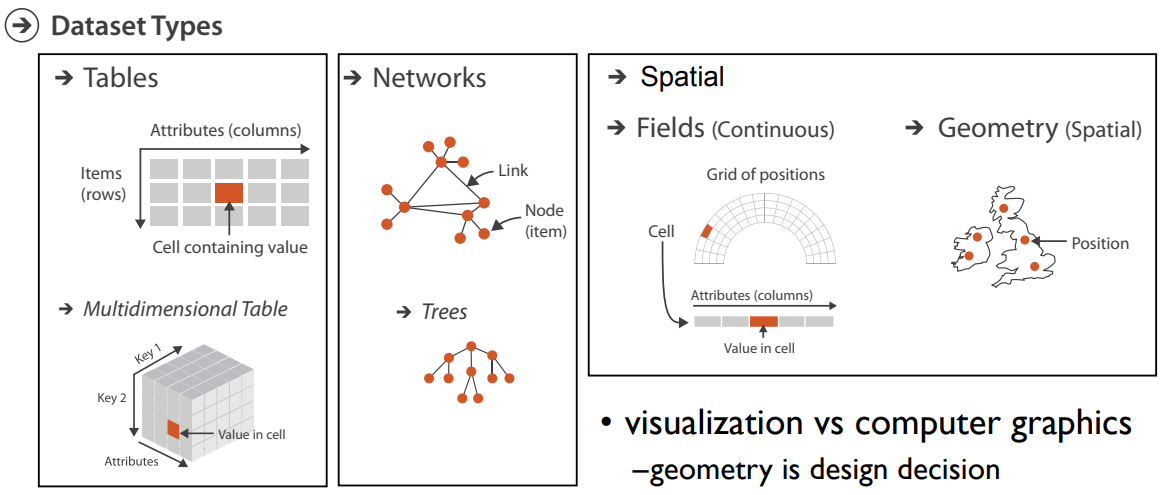
\includegraphics[width=1\linewidth]{figures/tmunzner_vad16} 

}

\caption{Dataset types, (Munzner 2014)}\label{fig:datasetTypes}
\end{figure}

Consider ploting 2 variables as an XY scatterplot. To add a 3rd variable append a z-axis othogonal (right angle to) the XY plane. Adding a 4th dimension is not so easily solved. Scatterplot matrices (SPLOM)(Chambers et al. 1983) plot every combination of variable pairs and views them in a matrix. This beats no visualization, but is not the ideal solution. Consider a small, square aquarium. Given 3 still frames of the variable-pair (that is, a square-on view from each dimension) does not accurately portray all of the information. For instance, a three-quarter (3/4) perspective helps relate the square on images and are ubiquitous in assembly and machining instustions. This perspective relates information contained in the view of sides. Mathematically, we describe the angle of view as a \texttt{basis}. Bases (plural of basis) are depicted as unit axes, they point in the direction each dimension is oriented. The axes for the three-quarter perspective is different from the square-on views in that the directions are a combination of 2 and 3 variables respectively, rather than one variable mapped fully to the horizontal or vertical.

\hypertarget{summary-of-research}{%
\subsection{Summary of research}\label{summary-of-research}}

\hypertarget{movition}{%
\subsection{Movition}\label{movition}}

\hypertarget{research-aim}{%
\subsection{Research aim}\label{research-aim}}

\hypertarget{methodology}{%
\subsection{Methodology}\label{methodology}}

\hypertarget{since-confirmation}{%
\section{Since Confirmation}\label{since-confirmation}}

\hypertarget{spinifex-app}{%
\subsection{Spinifex app}\label{spinifex-app}}

\hypertarget{multivate-linear-projection-study}{%
\subsection{Multivate linear projection study}\label{multivate-linear-projection-study}}

\hypertarget{thesis-structure}{%
\section{Thesis structure}\label{thesis-structure}}

\hypertarget{publications}{%
\section{Publications}\label{publications}}

\hypertarget{spinifex-package-r-journal}{%
\subsection{spinifex package (R Journal)}\label{spinifex-package-r-journal}}

\hypertarget{multivate-linear-projection-study-iee-vast}{%
\subsection{Multivate linear projection study (IEE VAST)}\label{multivate-linear-projection-study-iee-vast}}

\hypertarget{aim-3}{%
\subsection{Aim 3}\label{aim-3}}

\hypertarget{references}{%
\section*{References}\label{references}}
\addcontentsline{toc}{section}{References}

\hypertarget{refs}{}
\leavevmode\hypertarget{ref-anscombe_graphs_1973}{}%
Anscombe, F. J. 1973. ``Graphs in Statistical Analysis.'' \emph{The American Statistician} 27 (1): 17--21. \url{https://doi.org/10.2307/2682899}.

\leavevmode\hypertarget{ref-chambers_graphical_1983}{}%
Chambers, J. M., W. S. Cleveland, B. Kleiner, and P. A. Tukey. 1983. ``Graphical Methods for Data Analysis.''

\leavevmode\hypertarget{ref-matejka_same_2017}{}%
Matejka, Justin, and George Fitzmaurice. 2017. ``Same Stats, Different Graphs: Generating Datasets with Varied Appearance and Identical Statistics Through Simulated Annealing.'' In \emph{Proceedings of the 2017 CHI Conference on Human Factors in Computing Systems - CHI '17}, 1290--4. Denver, Colorado, USA: ACM Press. \url{https://doi.org/10.1145/3025453.3025912}.

\leavevmode\hypertarget{ref-munzner_visualization_2014}{}%
Munzner, Tamara. 2014. \emph{Visualization Analysis and Design}. AK Peters/CRC Press.

\leavevmode\hypertarget{ref-tukey_exploratory_1977}{}%
Tukey, John W. 1977. \emph{Exploratory Data Analysis}. Vol. 32. Pearson.


\end{document}
